\documentclass{article}
\usepackage{amsmath}
\usepackage[utf8]{inputenc}
\usepackage{graphicx}
\usepackage{verbatim}
\usepackage{float}
\usepackage[makeroom]{cancel}
\usepackage[english]{babel}
\usepackage{textcomp}
\usepackage{gensymb}
\usepackage{color}
\usepackage{subcaption}
\usepackage{caption}
\usepackage{hyperref}
\usepackage{physics}
\usepackage{dsfont}
%\usepackage{amsfonts}
\usepackage{listings}
\usepackage{multicol}
\usepackage{units}

% From Eirik's .tex
\usepackage{epstopdf}
\usepackage{cite}
\usepackage{braket}
\usepackage{url}
\bibliographystyle{plain}

\usepackage{algorithmicx}
\usepackage{algorithm}% http://ctan.org/pkg/algorithms
\usepackage{algpseudocode}% http://ctan.org/pkg/algorithmicx

\usepackage[margin=1cm]{caption}
\usepackage[outer=1.2in,inner=1.2in]{geometry}
% For writing full-size pages
%\usepackage{geometry}
%\geometry{
%  left=5mm,
%  right=5mm,
%  top=5mm,
%  bottom=5mm,
%  heightrounded,
%}

% Finding overfull \hbox
\overfullrule=2cm

\lstset{language=IDL}
 %\lstset{alsolanguage=c++}
\lstset{basicstyle=\ttfamily\small}
 %\lstset{backgroundcolor=\color{white}}
\lstset{frame=single}
\lstset{stringstyle=\ttfamily}
\lstset{keywordstyle=\color{red}\bfseries}
\lstset{commentstyle=\itshape\color{blue}}
\lstset{showspaces=false}
\lstset{showstringspaces=false}
\lstset{showtabs=false}
\lstset{breaklines}
\lstset{aboveskip=20pt,belowskip=20pt}

\lstset{basicstyle=\footnotesize, basewidth=0.5em}
\lstdefinestyle{cl}{frame=none,basicstyle=\ttfamily\small}
\lstdefinestyle{pr}{frame=single,basicstyle=\ttfamily\small}
\lstdefinestyle{prt}{frame=none,basicstyle=\ttfamily\small}
% \lstinputlisting[language=Python]{filename}


\definecolor{codepurple}{rgb}{0.58,0,0.82}
\definecolor{backcolour}{rgb}{0.95,0.95,0.92}
\definecolor{dkgreen}{rgb}{0,0.6,0}
\definecolor{gray}{rgb}{0.5,0.5,0.5}
\definecolor{magenta}{rgb}{0.58,0,0.82}

\lstdefinestyle{pystyle}{
  language=Python,
  aboveskip=3mm,
  belowskip=3mm,
  columns=flexible,
  basicstyle={\small\ttfamily},
  backgroundcolor=\color{backcolour},
  commentstyle=\color{dkgreen},
  keywordstyle=\color{magenta},
  numberstyle=\tiny\color{gray},
  stringstyle=\color{codepurple},
  basicstyle=\footnotesize,
  breakatwhitespace=false,
  breaklines=true,
  captionpos=b,
  keepspaces=true,
  numbers=left,
  numbersep=5pt,
  showspaces=false,
  showstringspaces=false,
  showtabs=false,
  tabsize=2
}

%%%%%%%%%%%%%%%%%%%%%%%%%%%%%%%%
% Self made macros here yaaaaaay
\newcommand\answer[1]{\underline{\underline{#1}}}
\newcommand\pd[2]{\frac{\partial #1}{\partial #2}}
\newcommand\red[1]{\textcolor{red}{\textbf{#1}}}
\newcommand\numberthis{\addtocounter{equation}{1}\tag{\theequation}}
% Usage: \numberthis \label{name}
% Referencing: \eqref{name}

% Some matrices
\newcommand\smat[1]{\big(\begin{smallmatrix}#1\end{smallmatrix}\big)}
\newcommand\ppmat[1]{\begin{pmatrix}#1\end{pmatrix}}

%%%%%%%%%%%%%%%%%%%%%%%%%%%%%%%%%
% Eirik's self made macros
\newcommand{\s}{^{*}}
\newcommand{\V}[1]{\mathbf{#1}}
\newcommand{\husk}[1]{\color{red} #1 \color{black}}
\newcommand{\E}[1]{\cdot 10^{#1}}
\newcommand{\e}[1]{\ \text{#1}}
\newcommand{\tom}[1]{\big( #1 \big)}
\newcommand{\Tom}[1]{\Big( #1 \Big)}
\newcommand{\tomH}[1]{\big[ #1 \big] }
\newcommand{\TomH}[1]{\Big[ #1 \Big]}
\newcommand{\tomK}[1]{ \{ #1 \} }
\newcommand{\TomK}[1]{\Big\lbrace #1 \Big\rbrace}
\newcommand{\bigabs}[1]{\left| #1 \right|}

% Section labeling
\usepackage{titlesec}% http://ctan.org/pkg/titlesec
\renewcommand{\thesubsection}{\arabic{subsection}}


% Title/name/date
\title{FYS4150 - Project 3}
\author{Simen Nyhus Bastnes \& Eirik Ramsli Hauge}
\date{24. October 2016}

\begin{document}
\maketitle
\begin{abstract}
In this project we will use Euler's forward method and Velocity Verlet to simulate the solar-system from given initial values. We will start off by looking at a solar system which only contains the Earth and the Sun, and then expand it by including other planets, starting with Jupiter. We will also include tests for conservation of kinetic energy, potential energy and angular momentum and find the escape velocity of an Earth like planet in the single planet solar system. Lastly, we will add a general relativistic correction to the gravitational force, and compare the perihelion angle with that given from classical Newtonian gravitation. We found that \husk{Write results summary}
\end{abstract}
\subsection{Introduction}
Differential equations are a big part of physics, and one of the most known differential equation can be said to be Newtons second law of motion. Many of our known differential equations can not be solved analytically for more than a few special cases. However, with the advent of computers, we are able to solve increasingly complex differential equations with no analytical solution, numerically\red{i dont like sentence, tried rewriting, failed, and needs to be looked at later}. To be able to solve differential equations numerically is therefore a great tool for any physicist and this project is designed to give us a basic understandig of how to solve a differential equation and as a bonus, how to use object orientation in C++. \\ \\
Our aim with this project is to simulate an entire solar system with the two methods forward Euler and Velocity Verlet. We will start with a system only containing the Sun and the Earth to compare our two methods. Afterwards we will run a test to see if the values for kinetic energy, potential energy and angular momentum are conserved. Thirdly we will see if we can find the escape velcoity of the Earth with trial and error and check if the velocity coincides with our analytical escape velocity. \\\\
The Sun-Earth system will be the basis for the rest of our solar system. When we are sure the smaller system works, we will add more planets (and Pluto) starting with Jupiter. Using object orientation and the fact that only the gravitational force is acting between the celestial bodies, we will find the sum of all forces working on a celestial body from the other celestial bodies. By accessing initial conditions from NASA we will relatively accurately simulate the whole solar system, which is pretty cool. \\\\
In the final part of the project we will add a general relativistic correction to the gravitational force, and compare the perihelion angle between the classic and the relativistic corrected case for the Sun-Mercury system. %Einstein's theory of general relativity predicts that this difference is about 43 arcseconds after a century.
If the difference is about 43 arcseconds after a century, we will have affirmed Einsteins theory of general relativity. Which is also pretty cool.
\subsection{Theory}
The goal of this project, is to develop a model of our solar system using the so-called velocity Verlet algorithm for solving coupled ordinary differential equations. For our solar system model, the only force interacting on it is gravity.
\subsubsection{The Earth-Sun system}
To start off, we simplify by looking at a hypothetical solar system with only the Earth orbiting around the Sun, where any solar motion is small enough to be neglected. Since the only force working on the system is the gravitational force between the Sun and the Earth, Newton's law of gravitation gives us that
\begin{align*}
F_G &= \frac{GM_{\odot}M_{\text{E}}}{r^2}
\intertext{where $M_{\odot}$ is the solar mass, $M_{\text{E}}$ is the mass of the Earth, $G$ the gravitational constant, and $r$ is the distance between the Earth and the Sun. Written on vector form, $F_G$ takes the following form}
  F_{G,\mathbf{r}} &= -\frac{GM_{\odot}M_{\text{E}}}{r^3}\,\mathbf{r}
\end{align*}
where $\mathbf{r} = x\mathbf{i}+y\mathbf{j}+z\mathbf{k}$ is the vector from the Sun to the Earth.
\begin{align*}
F_{G,\mathbf{r}} &= -\frac{GM_{\odot}M_{\text{E}}}{r^3}\,(x\mathbf{i}+y\mathbf{j}+z\mathbf{k})\numberthis\label{eq:FG_comp}
\end{align*}
\\Using Newton's second law of motion, we can then get the following differential equations for the motion of the Earth.
\begin{align*}
\frac{d^2x}{dt^2} = \frac{F_{G,x}}{M_{E}}\numberthis\label{eq:diffx}\\
\frac{d^2y}{dt^2} = \frac{F_{G,y}}{M_{E}}\numberthis\label{eq:diffy}\\
\frac{d^2z}{dt^2} = \frac{F_{G,z}}{M_{E}}\numberthis\label{eq:diffz}
\end{align*}
where $F_{G,x}$, $F_{G,y}$, and $F_{G,z}$ are the components of the gravitational force, given by \eqref{eq:FG_comp}. We can assume that the orbit of the Earth (and other objects in the solar system) around the Sun is mostly co-planar, so we could take this to be the $xy$-plane, reducing our differential equations to equations \eqref{eq:diffx} and \eqref{eq:diffy}. However, since looking at the system in three dimensions isn't that much more work, we will continue doing so.\\\\
We can obtain mass units from assuming that the Earth's orbit is almost circular around the Sun. For circular motion, we know that the force obeys the following relation
\begin{align*}
F_G &= \frac{M_{\text{E}}v^2}{r} = \frac{GM_{\odot}M_{\text{E}}}{r^2}
\end{align*}
where $v$ is the velocity of the Earth. This can be shown to give us the useful relation
\begin{align*}
  v^2r = GM_{\odot} = 4\pi^2\text{AU}^3/\text{yr}^2\numberthis\label{eq:mass_units}
\end{align*}
which we can use to scale both distance and time units to more ideal orders of magnitudes. One astronomical unit (1 AU) is defined as the average distance from the Earth to the Sun, or roughly $10^{11}$ m. Inserting this into equation \eqref{eq:FG_comp}, gives us
\begin{align*}
F_{G,\mathbf{r}} &= \frac{4\pi^2\text{AU}^3/\text{yr}^2\,M_{\text{E}}}{r^3}(x\mathbf{i}+y\mathbf{j}+z\mathbf{k})
\end{align*} 
where $r$ now is given in units AU, and time is given in years. Using years instead of seconds matches the time evolution of our solar system better, as the Earth for example orbits the Sun once per year.
By looking at equation \eqref{eq:mass_units}, we realize that the velocity required for circular orbit falls out
\begin{align*}
  v_{\text{circ}}^2r &= 4\pi^2\text{AU}^3/\text{yr}^2\\
  v_{\text{circ}} &=2\pi\sqrt{\frac{\text{AU}^3}{r}}\,\text{yr}^{-1}\numberthis\label{eq:v_circ}
\end{align*}
For our Earth, which lies at $r = 1$ AU, equation \eqref{eq:v_circ} gives us $v_{\text{circ}} = 2\pi$.\\\\
The total energy of the Earth can be given as $E_{\text{tot,E}} = T_{\text{E}} + U_{\text{E}}$, where
\begin{align*}
  T_{\text{E}} &= \frac{1}{2}M_{\text{E}}v_{\text{E}}^2
  \intertext{is the kinetic energy for the Earth, and the potential energy is $U$ of the Earth in our system given as}
  U_{\text{E}} &= \frac{GM_{\odot}M_{\text{E}}}{r}\\
  &= \frac{4\pi^2\text{AU}^3/\text{yr}^2\,M_{\text{E}}}{r}
\end{align*}
where $r$ is the distance given in AU. From this we can find the escape velocity, which is the initial velocity an object needs to escape from its orbit. This occurs when the kinetic energy is equal the potential energy. For the Earth, this is
\begin{align*}
  T_{\text{E}} &= U_{\text{E}}\\
  \frac{1}{2}M_{\text{E}}v_{\text{esc}}^2 &= \frac{GM_{\odot}M_{\text{E}}}{r}\\
  v_{\text{esc}} &= \sqrt{\frac{2GM_{\odot}}{r}}\numberthis\label{eq:v_esc}
  \intertext{Inserting $r = 1$ AU and our result from equation \eqref{eq:mass_units}, we get}
  v_{\text{esc}} &= 2\sqrt{2}\,\pi\,\text{AU}/\text{yr}
\end{align*}
or expressed in terms of the circular orbit velocity $v_{\text{esc}} = \sqrt{2}\,v_{\text{circ}}$.\\\\
In order to solve the differential equations (equations \eqref{eq:diffx}, \eqref{eq:diffy}, and \eqref{eq:diffz}) numerically, we need to discretize them. For simplicity, we will only derive the discretized expression for the $x$-direction, though the derivation is the same for the other directions. In the non-discretized situation, the position of an object in the $x$-direction is given by $x(t)$, where $t$ is the time. We start by discretizing the time by defining the time steps $t_i$ in the interval $t_1 \dots t_n$, so
\begin{align*}
  t_i =  t_1 +  ih
\end{align*}
where $h$ is the step length and $i = 0,1,\dots,n$, so that we can write $t_{i+1} = t_i + h$. Now, we can write $x(t)$ in terms of the discretized time, $x(t_i)$. We can simplify the notation by writing $x(t_i)$ as $x_i$. Inserting this into equation \eqref{eq:FG_comp} gives us
\begin{align*}
  F_{G,x_i} &= -\frac{GM_{\odot}M_{\text{E}}}{r^3}\,x_i
\end{align*}
We then get the discretized differential equation for $x$ from equation \eqref{eq:diffx} 
\begin{align*}
  x_i'' &= -\frac{GM_{\odot}}{r^3}x_i
\end{align*}
Or when inserting the expression for $GM_{\odot}$ from equation \eqref{eq:mass_units}
\begin{align*}
  x_i'' &= -\frac{4\pi^2 \text{AU}^3/\text{yr}^2}{r^3}\,x_i \numberthis\label{eq:discx}
\end{align*}
\subsubsection{Numerical methods for solving ordinary differential equations}
Euler's forward method \cite{Euler} is a well known numerical method used to solve differential equations. The method is fairly simple, basing itself on that the next step is the former step added with its own derivative times a steplength. By defining $h$ as the step length we can write express Euler's forward method as follows:
\begin{equation}
f_{i + 1} = f_i + f^{'}_i \cdot h
\label{eq:fwdEuler}
\end{equation}
where we define $f_i$ as $f(i)$, $f_{i+1} = f(i + h)$ and $i = 0, 1, 2 ... , n$. \\
In our case we use Newton's laws and we want to find the position and velocity of our celestial bodies. Since it's easy to find the acceleration from equation \eqref{eq:FG_comp}, and we know that $a = \frac{\partial^2 x}{\partial t^2}$ and $v = \frac{\partial x}{\partial t}$ where $x$ is position, $v$ is velocity and $a$ is acceleration, Euler's forward method becomes:
\begin{equation}
v_{i + 1} = v_i + h \cdot a_i + \mathcal{O}(h^2)\\
\label{eq:Eulervel}
\end{equation}
\begin{equation}
x_{i + 1} = x_i + h \cdot v_i + \mathcal{O}(h^2)\\
\label{eq:Eulerpos}
\end{equation}
We can implement the algorithm as follows:
\begin{algorithm}[H]
\small
\caption{Forward Euler}\label{alg:VelVerlet}
\begin{algorithmic}[1]
\For{$i = 0, n$}
\State $v_{i+1} = v_i + h\cdot a_i $
\State $x_{i+1} = x_i + h\cdot v_i $
\EndFor
\end{algorithmic}
\end{algorithm}
Where we calculate $F_{G, r_i}$ with equation \eqref{eq:FG_comp}.By counting we can see that this gives us 4n FLOPs. \\ \\
The Verlet Velocity method presents a different approach to solve the differential equations in this project. While Euler's method is applicable to many differential equations, the Verlet methods are specified to solve Newton's equations of motion \cite{Newton}. The Verlet Velocity method is derived by first Taylor expanding $x_{i + 1}$ ad $x_{i-1}$:
\begin{align*}
x_{i-1} &\simeq x_i - v_i h + \frac{1}{2}a_i h^2 \\
x_{i+1} &\simeq x_i + v_i h + \frac{1}{2}a_i h^2
\intertext{By adding the two expressions we can find an expression for $x_{i+1}$}
x_{i+1} + x_{i-1} &= 2x_i + a_i h^2 \\
x_{i+1} &= 2x_i - x_{i-1} + a_i h^2 \\
\intertext{and by subtracting them we can find an expression for $v_{i}$}
x_{i+1} - x_{i-1} &= 2h v_i \\
v_i &= \frac{x_{i+1} - x_{i-1}}{2h}
\intertext{These expressions for $x_{i+1}$ and $v_i$ are called the Verlet method. However, we want to have an expression for $v_{i+1}$.}
v_{i+1} &= \frac{x_{i+2} - x_i}{2h} \\
\intertext{We can easily find $x_{i+1}$ by using the expression above}
x_{i+2} &= 2x_{i+1} - x_i + a_{i+1} h^2 \\
\intertext{Inserting this back into $v_{i+1}$ gives us:}
v_{i+1} &= \frac{2x_{i+1} - x_i + a_{i+1} h^2 - x_i}{2h} \\
v_{i+1} &= \frac{x_{i+1} - x_i}{h} + \frac{1}{2} a_{i+1} h
\intertext{Inserting the Taylor expanded $x_{i+1}$ for $v_i$ dependency}
v_{i+1} &= \frac{x_i + v_i h + \frac{1}{2} a_i h^2 - x_i}{h} + \frac{1}{2} a_{i+1} h \\
v_{i+1} &= v_i + \frac{1}{2} a_i h + \frac{1}{2} a_{i+1} h \\
\end{align*}
This gives us the equations for position and velocity in the velocity Verlet method:
\begin{equation}
x_{i+1} = x_i + v_i h + \frac{1}{2} a_i h^2 + \mathcal{O}(h^3)
\label{eq:Verletpos}
\end{equation}
\begin{equation}
v_{i+1} = v_i + \frac{1}{2} h (a_i + a_{i+1}) + \mathcal{O}(h^3)
\label{eq:Verletvel}
\end{equation}
As we can see, the term for $v_{i+1}$ is dependent on $a_{i+1}$. Therefore the algorithm must go like this:
\begin{algorithm}[H]
\small
\caption{Velocity Verlet}\label{alg:VelVerlet}
\begin{algorithmic}[1]
\For{$i = 0, n$}
\State $r_{i+1} = r_i + v_i h + \frac{1}{2} a_i h^2$
\State $a_{i+1} = F_{G, r_{i+1}}/m$
\State $v_{i+1} = v_i + \frac{1}{2} h (a_i + a_{i+1})$
\EndFor
\end{algorithmic}
\end{algorithm}
Where we calculate $F_{G, r}$ with euation \eqref{eq:FG_comp}. By counting we can see that we have 11 FLOPs  which is a bit more than the double of forward Euler. \husk{Should we change to the one we actually use?}

\subsubsection{The three-body problem}
\red{adding jupyter}

\subsubsection{Perihelion precession}
Lastly we want to study the perihelion angle of Mercury. This was an important test of the general relativity. When one compared the observed value of the perhelion precession to all classical effects, there was a difference of about 43 arcseconds after a century. This difference was not understood until Einstein predicted it with general relativity.\cite{Perhelion} Einstein found that the perihelion precession could be predicted by:
\begin{equation}
\epsilon = 24 \pi^3 \frac{\alpha^2}{T^2 c^2 (1 - e^2)}
\label{eq:perihelion}
\end{equation}
Where $\alpha$ is the major semi-axis of the planets orbit, $e$ is the eccentricity of the orbit, $T$ the period of revolution and $c$ the speed of light. By inserting the right values for Mercury, it was found that for a year the precession was about 0.104 arcseconds and after a (Earth) century, Mercury would have revolved about 415 times around the sun giving a precession of about 43 arcseconds which coincides with the difference between the observed and classically calculated value thus proving general relativity. \\
It became clear that the Newtonian force of gravity needed a relativistic correction. In our numerical calculations, we will therefore add a correction setting the gravitational force to:
\begin{equation}
F_G = \frac{G M_{\odot} M_{Mercury}}{r^2} \, \, \TomH{1 + \frac{3l^2}{r^2c^2}}
\label{eq:FgGR}
\end{equation}
Where $l$ is the orbital angular momentum given as $l = |\vec{r} \cross \vec{v}|$ for Mercury and $c$ is once again the speed of light.
We can then find the perihelion angle by
\begin{equation}
\tan \theta_p = \frac{y_p}{x_p}
\end{equation}
where $y_p$ and $x_p$ are $y$ and $x$ respectively at perihelion.
\subsection{Experimental}
The programs used in this project can be found in the GitHub repository \cite{Github}, in the \texttt{/src/} folder. When running the program, it takes 4 command line arguments, \texttt{task}, $dt$, \texttt{task parameter} and \texttt{method}. The program has four different runmodes, which we will discuss in some more detail. All data written to file by the program are stored in \texttt{/benchmarks/} with different subfolders for each runmode.
\subsubsection*{The Earth-Sun system}
Setting \texttt{task} to \texttt{ES} runs the program for a two-body solar system containing the Earth and the Sun which is fixed in origo. The Earth starts at a distance of 1 AU from the Sun along  the x-axis and \texttt{task parameter} gives its initial velocity in the y-direction. \texttt{Method} can be set to either \texttt{Euler} or \texttt{Verlet} for using either forward Euler or Velocity Verlet . The position vectors of the Sun and the Earth are saved in the file \texttt{ES/pos\_<method>\_dt<dt>\_N<number of timesteps>\_vy<initial velocity in y-direction>.xyz}\\ where everything inside a \texttt{<>} means the value given for that run through.
\subsubsection*{The Earth-Sun-Jupiter system}
Setting \texttt{task} to \texttt{ESJ1} runs the program for a three-body solar system containing the Earth, Jupiter and the Sun which is fixed in origo. Setting \texttt{task} to \texttt{ESJ2} sets origo as center-of-mass for the same system. \texttt{Task parameter} gives a factor to multpily with Jupiters mass. \texttt{Method} can be set to either \texttt{Euler} or \texttt{Verlet}. 
Positions of all celestial bodies are written to the file \\ \texttt{ESJ/pos\_dt<dt>\_N<number of timesteps>\_m<mass factor>.xyz}
\subsubsection*{The whole Solar System}
Setting \texttt{task} to \texttt{WS} runs the program for a solar system containing the Sun, all the planets and Pluto revolving around the centre of mass. \texttt{Task parameter} sets the number of years one wants the simulation to run. \texttt{Method} can be set to either \texttt{Euler} or \texttt{Verlet}. The position of all celestial bodies are written to the file \\ 
\texttt{WS/pos\_dt<dt>\_N<number of timesteps>.xyz}
\subsubsection*{Perhelion precession}
Setting \texttt{task} to \texttt{GR} runs the program for a two-body solar system containing Mercury and the Sun. \texttt{Task parameter} sets the number of years one wants the simulation to run. \texttt{Method} can be set to either \texttt{Euler}, \texttt{Verlet} or \texttt{VerletREL} where the latter uses Velocity Verlet with a relativistic correction to the gravitation force. The perhelion angle is saved to the file
\texttt{GR/ang\_per<method>\_dt<dt>}
\subsection{Results}
\subsubsection*{The Earth-Sun system}
By initializing a system containing the Earth and the Sun and simulating it using forward Euler with different time steps we got the plots shown in figure \ref{fig:ES-Euler}. And by doing the same only with Velocity Verlet we achieved the plots in figure \ref{fig:ES-Verlet}. 
%%%%%%%%%%%%%%%%%%%%%%%%%%%%%%%%%%
%%%           ES-Euler         %%%
%%%%%%%%%%%%%%%%%%%%%%%%%%%%%%%%%%
\begin{figure}[H]
\centering
\begin{subfigure}{0.32\textwidth}
	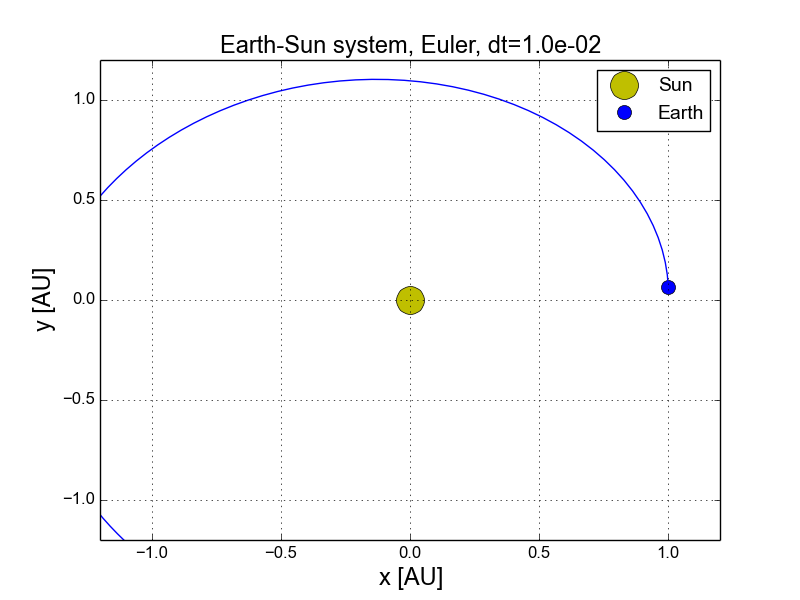
\includegraphics[scale=0.25]{{../figures/ES/ES_Euler_dt1.0e-02_vy6.28}.png}
	\caption{dt = 1.0e-02}
	\label{fig:eulerdt1.0e-02}
\end{subfigure}
\begin{subfigure}{0.33\textwidth}
	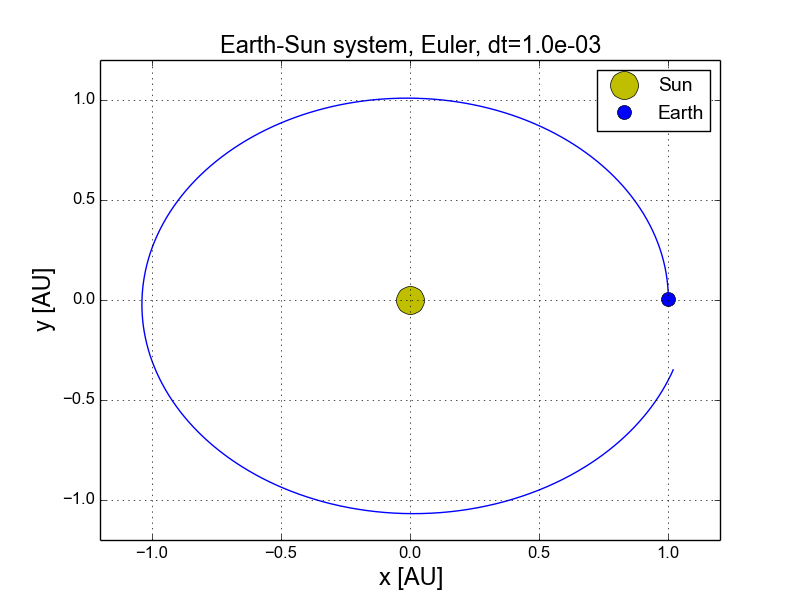
\includegraphics[scale=0.25]{{../figures/ES/ES_Euler_dt1.0e-03_vy6.28}.png}
	\caption{dt = 1.0e-03}
	\label{fig:eulerdt1.0e-03}
\end{subfigure}
\begin{subfigure}{0.33\textwidth}
	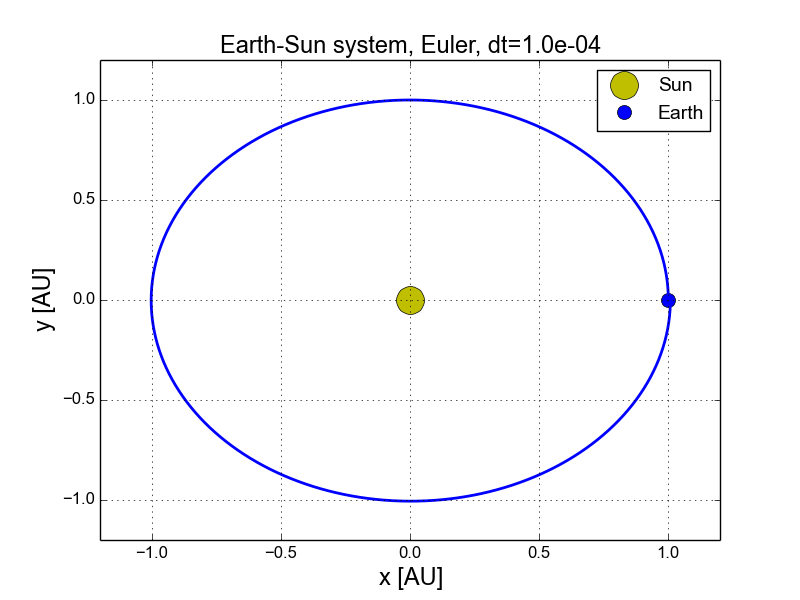
\includegraphics[scale=0.25]{{../figures/ES/ES_Euler_dt1.0e-04_vy6.28}.png}
	\caption{dt = 1.0e-04}
	\label{fig:eulerdt1.0e-04}
\end{subfigure}
\caption{Simulation of the Earth-Sun system using forward Euler with different time steps. The initial velocity is in all cases set to 6.28 AU/years, the Sun is fixed in origo and the Earth starts in (1, 0, 0) AU}
\label{fig:ES-Euler}
\end{figure}

%%%%%%%%%%%%%%%%%%%%%%%%%%%%%%%%%%
%%%          ES-Verlet         %%%
%%%%%%%%%%%%%%%%%%%%%%%%%%%%%%%%%%
\begin{figure}[H]
\centering
\begin{subfigure}{0.32\textwidth}
	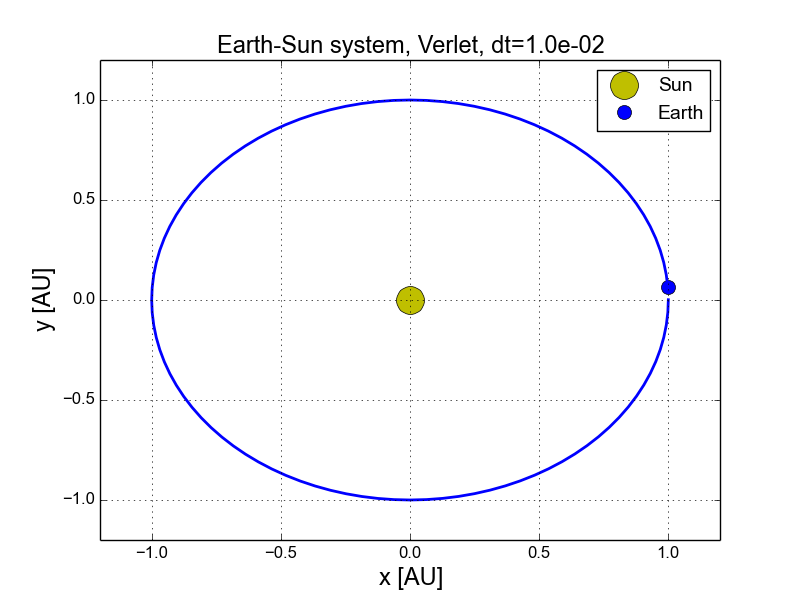
\includegraphics[scale=0.25]{{../figures/ES/ES_Verlet_dt1.0e-02_vy6.28}.png}
	\caption{dt = 1.0e-02}
	\label{fig:verletdt1.0e-02}
\end{subfigure}
\begin{subfigure}{0.33\textwidth}
	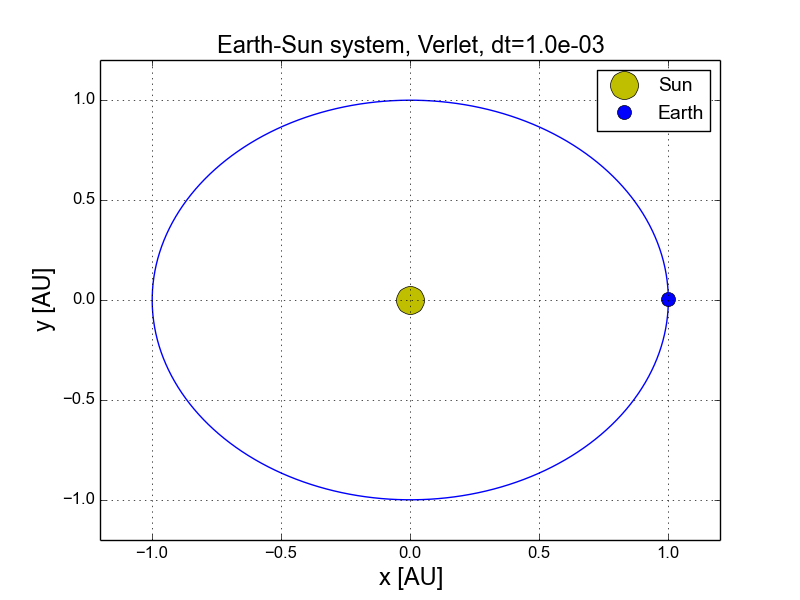
\includegraphics[scale=0.25]{{../figures/ES/ES_Verlet_dt1.0e-03_vy6.28}.png}
	\caption{dt = 1.0e-03}
	\label{fig:verletdt1.0e-03}
\end{subfigure}
\begin{subfigure}{0.33\textwidth}
	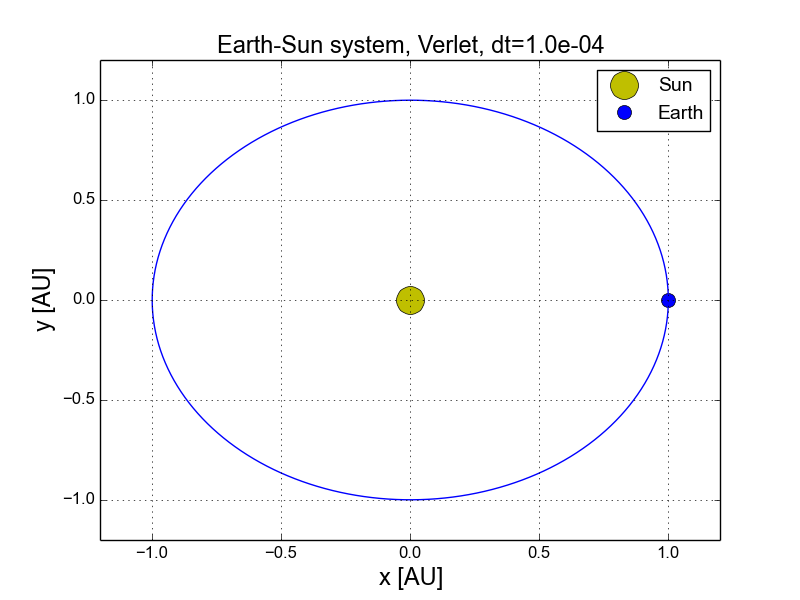
\includegraphics[scale=0.25]{{../figures/ES/ES_Verlet_dt1.0e-04_vy6.28}.png}
	\caption{dt = 1.0e-04}
	\label{fig:verletdt1.0e-04}
\end{subfigure}
\caption{Simulation of the Earth-Sun system using Velocity Verlet with different time steps. The initial velocity is in all cases set to 6.28 AU/years in the y-direction, the Sun is fixed in origo and the Earth starts in (1, 0, 0) AU}
\label{fig:ES-Verlet}
\end{figure}

%%%%%%%%%%%%%%%%%%%%%%%%%%%%%%%%%%
%%%          ES-escape         %%%
%%%%%%%%%%%%%%%%%%%%%%%%%%%%%%%%%%
Analytically we found that the escape velocity was 8.89 AU/years. Some of our trial and errors are shown in figure \ref{fig:ESe}:
\begin{figure}
\begin{subfigure}{0.32\textwidth}
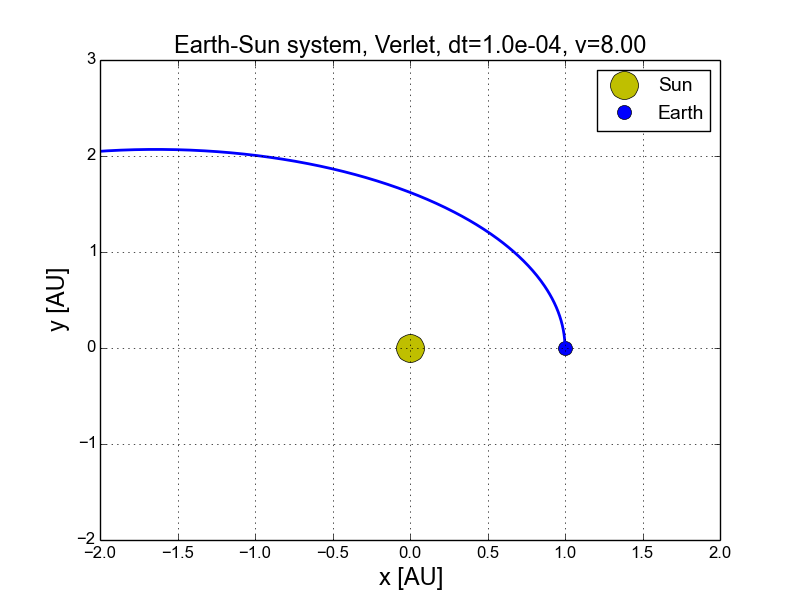
\includegraphics[scale=0.25]{{../figures/ES/ES_Verlet_dt1.0e-04_yrs2_vy8.00}.png}
\caption{$v = 8.00$ AU/years}
\label{fig:ESe8}
\end{subfigure}
\begin{subfigure}{0.33\textwidth}
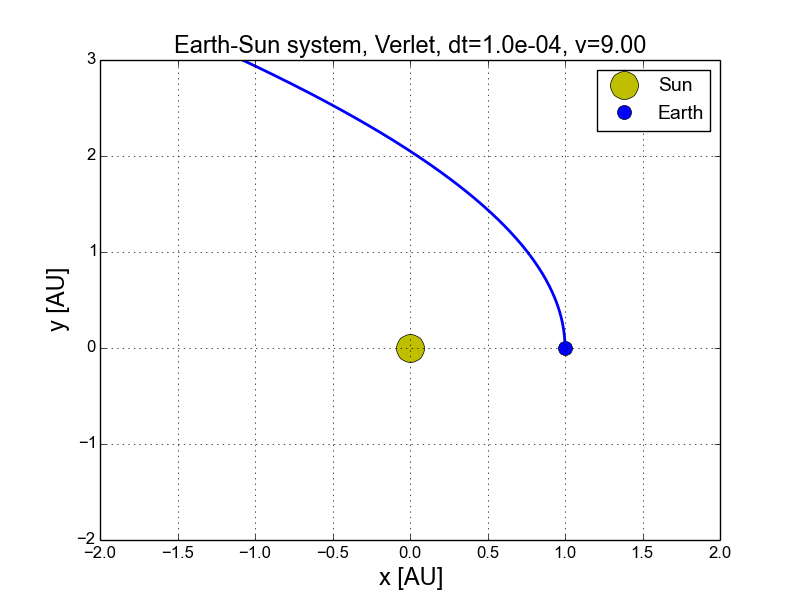
\includegraphics[scale=0.25]{{../figures/ES/ES_Verlet_dt1.0e-04_yrs2_vy9.00}.png}
\caption{$v = 9.00$ AU/years}
\label{fig:ESe9}
\end{subfigure}
\begin{subfigure}{0.33\textwidth}
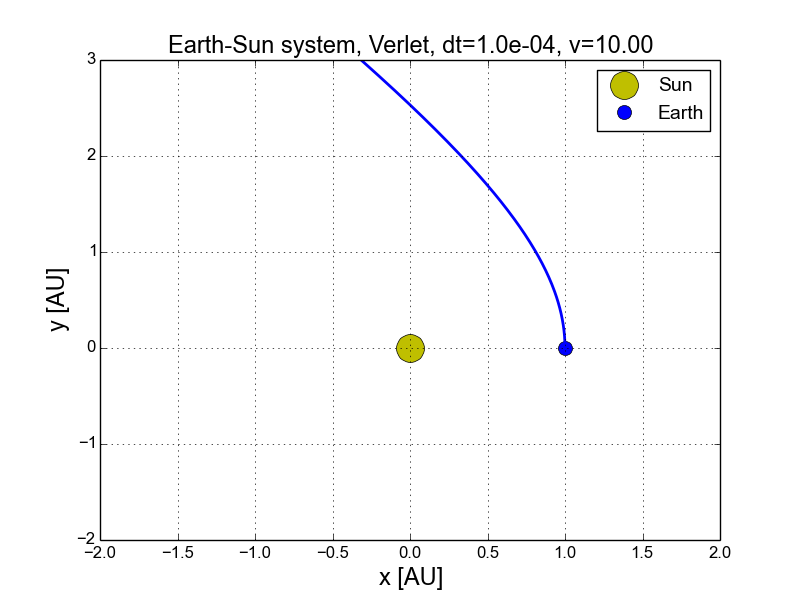
\includegraphics[scale=0.25]{{../figures/ES/ES_Verlet_dt1.0e-04_yrs2_vy10.00}.png}
\caption{$v = 10.00$ AU/years}
\label{fig:ESe10}
\end{subfigure}
\caption{Simulation of the Earth-Sun system using Velocity Verlet with different initial velocity for the Earth. The velocity is only in the y-direction. The Sun is fixed in origo and the Earth starts in (1, 0, 0) AU. Simulates a time period of two years.}
\label{fig:ESe}
\end{figure}
\subsubsection*{The Earth-Sun-Jupiter system}
Adding Jupiter to our system and keeping the Sun in origo we achieved the plots shown in figure \ref{fig:ESJ1}. By letting the Sun move around the center-of-mass, we got the plots in figure \ref{fig:ESJ2}. The plots in figure \ref{fig:ESJ1Crash} were drawn by letting the mass of Jupiter increase while the Sun was fixed in origo.
%%%%%%%%%%%%%%%%%%%%%%%%%%%%%%%%%%
%%%            ESJ1            %%%
%%%%%%%%%%%%%%%%%%%%%%%%%%%%%%%%%%
\begin{figure}[H]
\begin{subfigure}{0.32\textwidth}
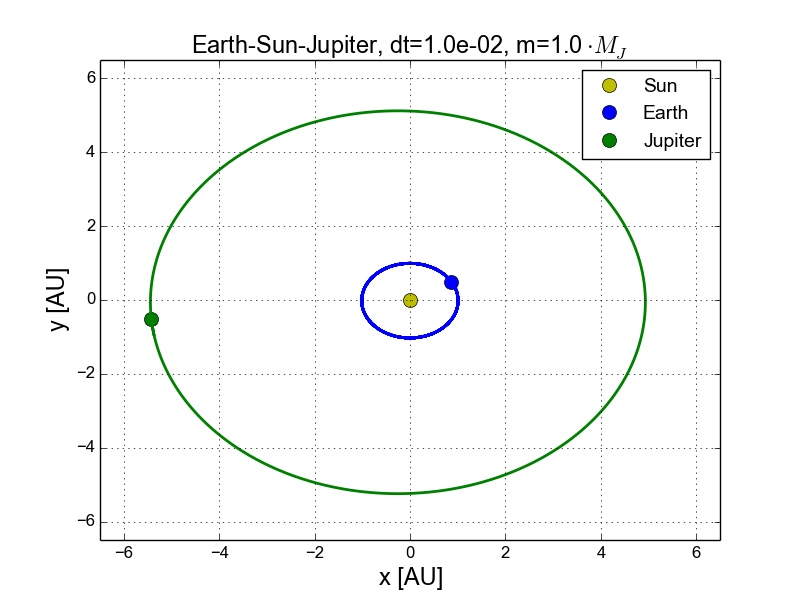
\includegraphics[scale=0.25]{{../figures/ESJ1/ESJ1_dt1.0e-02_m1.0}.png}
\caption{dt = 1.0e-02}
\label{fig:ESJ11.0e-02}
\end{subfigure}
\begin{subfigure}{0.33\textwidth}
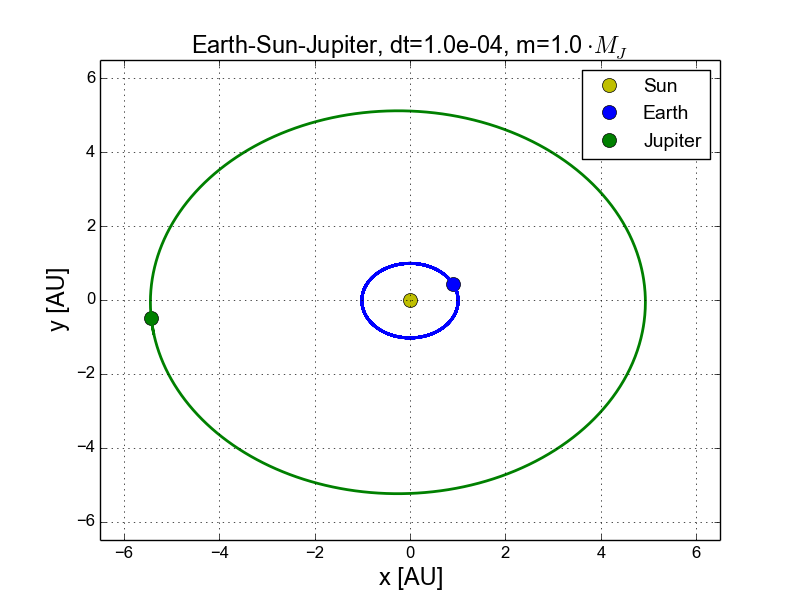
\includegraphics[scale=0.25]{{../figures/ESJ1/ESJ1_dt1.0e-04_m1.0}.png}
\caption{dt = 1.0e-04}
\label{fig:ESJ11.0e-04}
\end{subfigure}
\begin{subfigure}{0.33\textwidth}
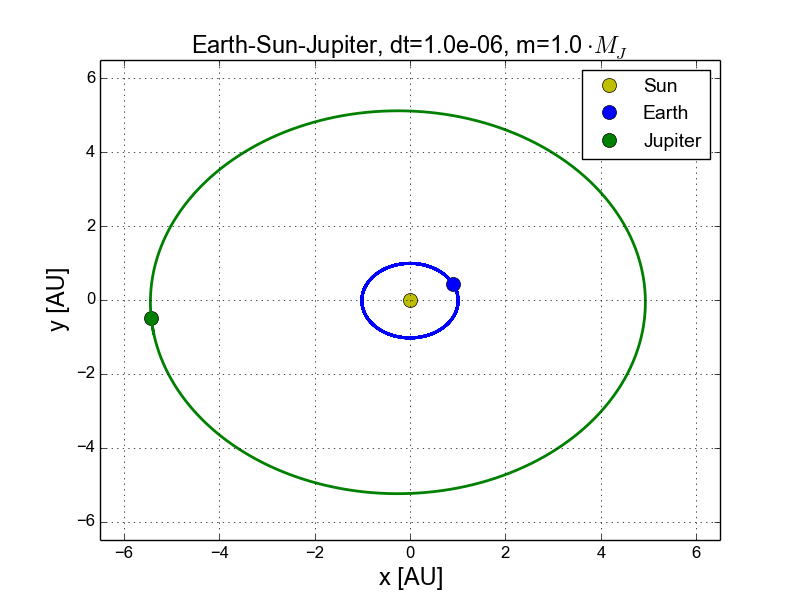
\includegraphics[scale=0.25]{{../figures/ESJ1/ESJ1_dt1.0e-06_m1.0}.png}
\caption{dt = 1.0e-06}
\label{fig:ESJ11.0e-06}
\end{subfigure}
\caption{Simulation of the Earth-Sun-Jupiter system using Velocity Verlet with different time steps. Initial velocity and position for the Earth and Jupiter are retrieved from NASA and the Sun is fixed to Origo.}
\label{fig:ESJ1}
\end{figure}

%%%%%%%%%%%%%%%%%%%%%%%%%%%%%%%%%%
%%%            ESJ2            %%%
%%%%%%%%%%%%%%%%%%%%%%%%%%%%%%%%%%
\begin{figure}[H]
\begin{subfigure}{0.32\textwidth}
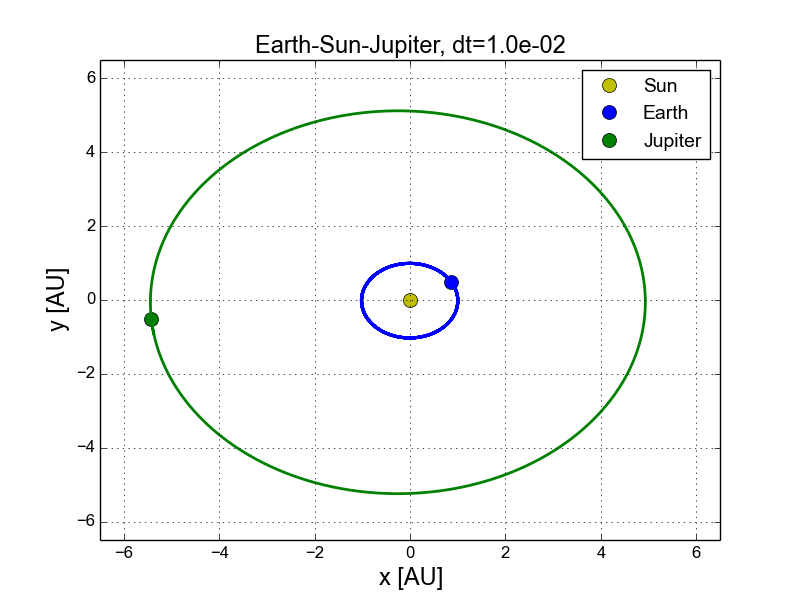
\includegraphics[scale=0.25]{{../figures/ESJ2/ESJ2_dt1.0e-02_m1.0}.png}
\caption{dt = 1.0e-02}
\label{fig:ESJ21.0e-02}
\end{subfigure}
\begin{subfigure}{0.33\textwidth}
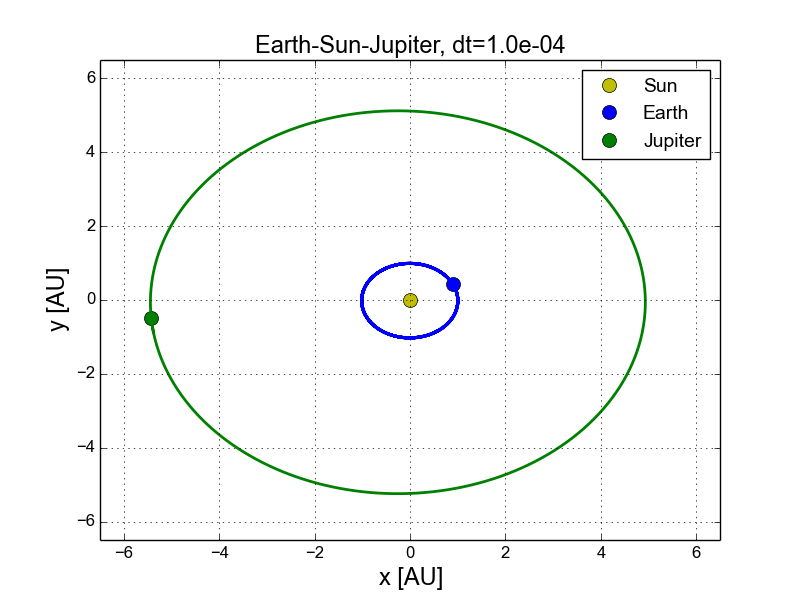
\includegraphics[scale=0.25]{{../figures/ESJ2/ESJ2_dt1.0e-04_m1.0}.png}
\caption{dt = 1.0e-04}
\label{fig:ESJ21.0e-04}
\end{subfigure}
\begin{subfigure}{0.33\textwidth}
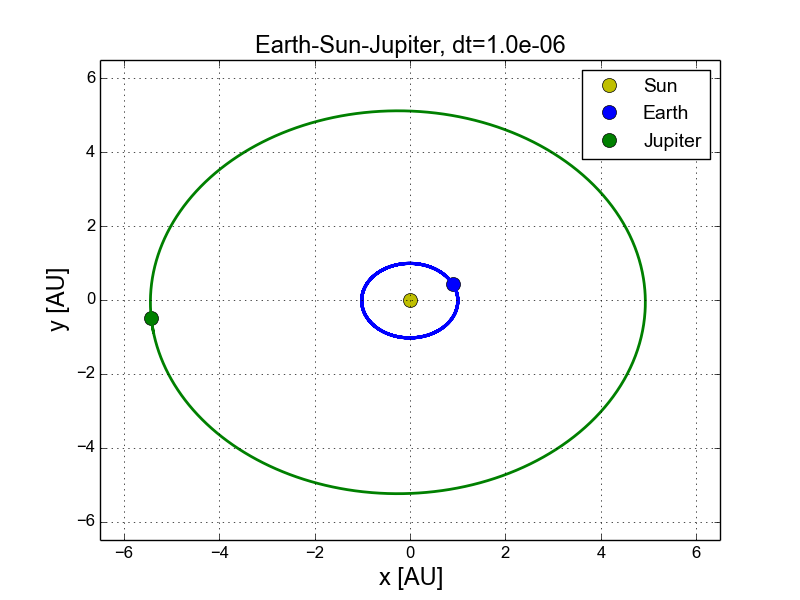
\includegraphics[scale=0.25]{{../figures/ESJ2/ESJ2_dt1.0e-06_m1.0}.png}
\caption{dt = 1.0e-06}
\label{fig:ESJ21.0e-06}
\end{subfigure}
\caption{Simulation of the Earth-Sun-Jupiter system using Velocity Verlet with different time steps. Initial velocity and position for the Earth, the Sun and Jupiter are retrieved from NASA and the center-of-mass is in origo.}
\label{fig:ESJ2}
\end{figure}

%%%%%%%%%%%%%%%%%%%%%%%%%%%%%%%%%%
%%%         ESJ-Crash          %%%
%%%%%%%%%%%%%%%%%%%%%%%%%%%%%%%%%%
\begin{figure}[H]
\begin{subfigure}{0.32\textwidth}
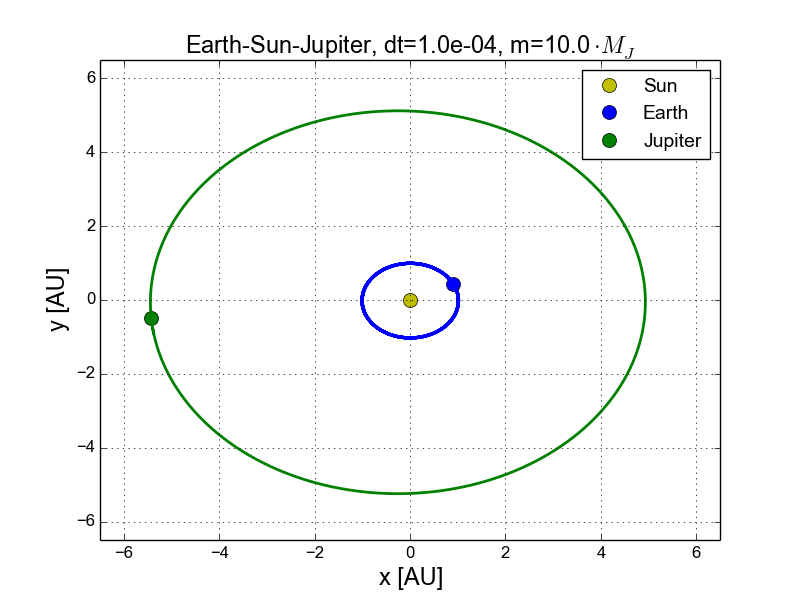
\includegraphics[scale=0.25]{{../figures/ESJ1/ESJ1_dt1.0e-04_m10.0}.png}
\caption{10 Jupiter masses}
\label{fig:ESJm10}
\end{subfigure}
\begin{subfigure}{0.33\textwidth}
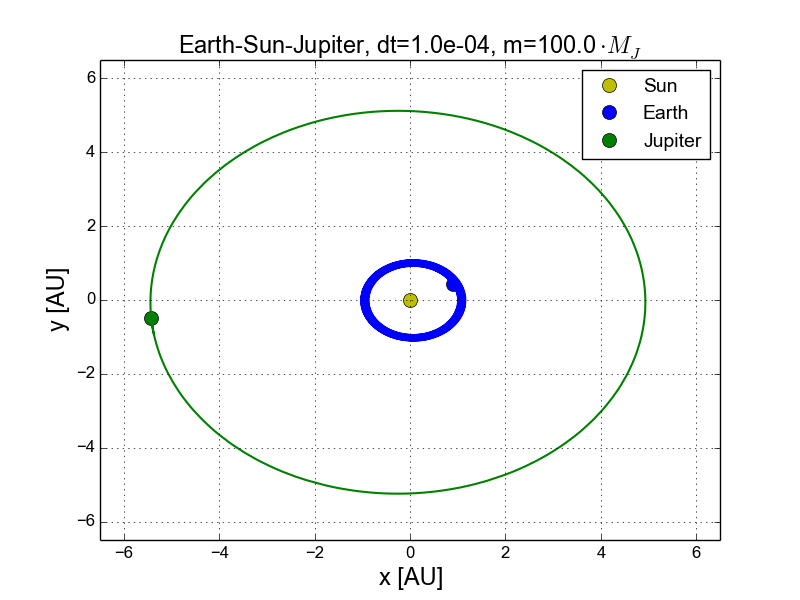
\includegraphics[scale=0.25]{{../figures/ESJ1/ESJ1_dt1.0e-04_m100.0}.png}
\caption{100 Jupiter masses}
\label{fig:ESJm100}
\end{subfigure}
\begin{subfigure}{0.33\textwidth}
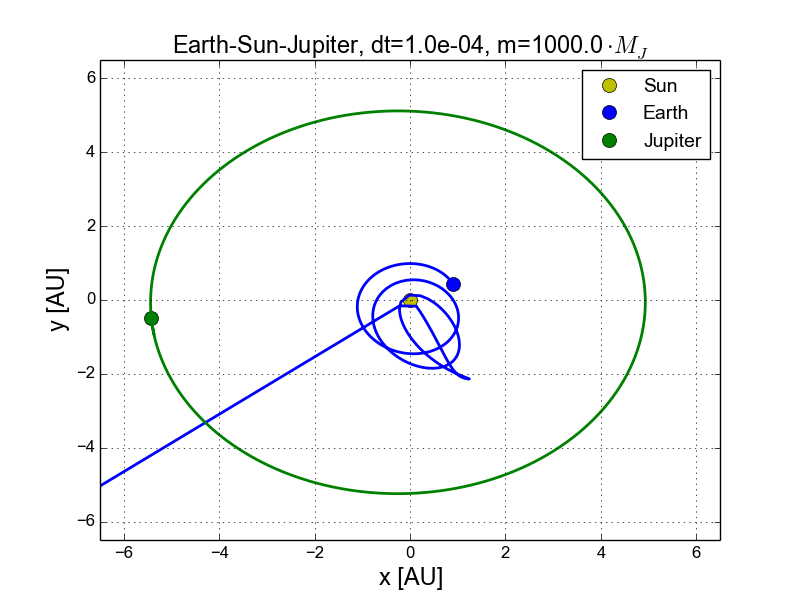
\includegraphics[scale=0.25]{{../figures/ESJ1/ESJ1_dt1.0e-04_m1000.0}.png}
\caption{1000 Jupiter masses}
\label{fig:ESJm1000}
\end{subfigure}
\caption{Simulation of the Earth-Sun-Jupiter system using Velocity Verlet with different mass of Jupiter. Initial velocity and position for the Earth and Jupiter are retrieved from NASA and the Sun is fixed to Origo.}
\label{fig:ESJ1Crash}
\end{figure}
\subsubsection*{The whole Solar System}
Simulating the Solar System with the Sun, all eight planets and Pluto gave us the results presented in figure \ref{fig:WS}
\begin{figure}[H]
\begin{subfigure}{0.32\textwidth}
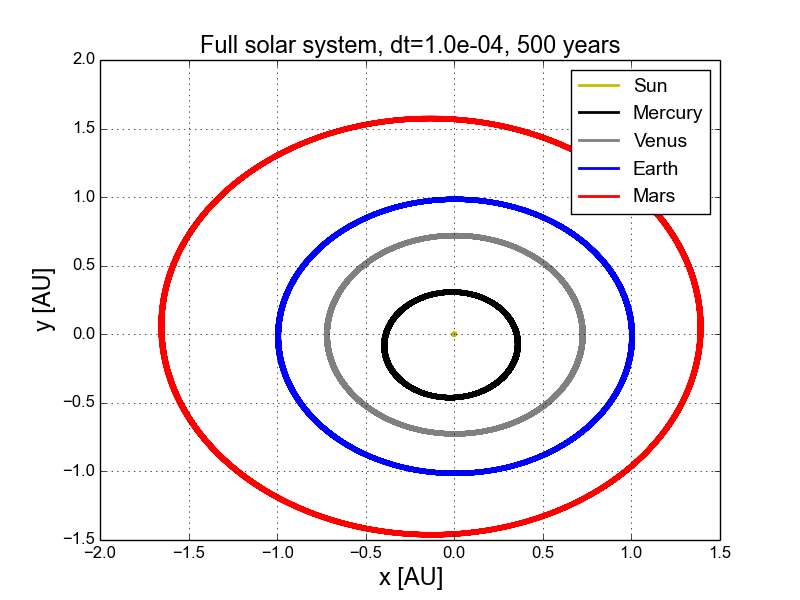
\includegraphics[scale=0.25]{{../figures/WS/pos05_dt1.0e-04_yrs500.0}.png}
\caption{Inner Solar System, $dt = 1.0e-04$}
\label{fig:WSISS}
\end{subfigure}
\begin{subfigure}{0.33\textwidth}
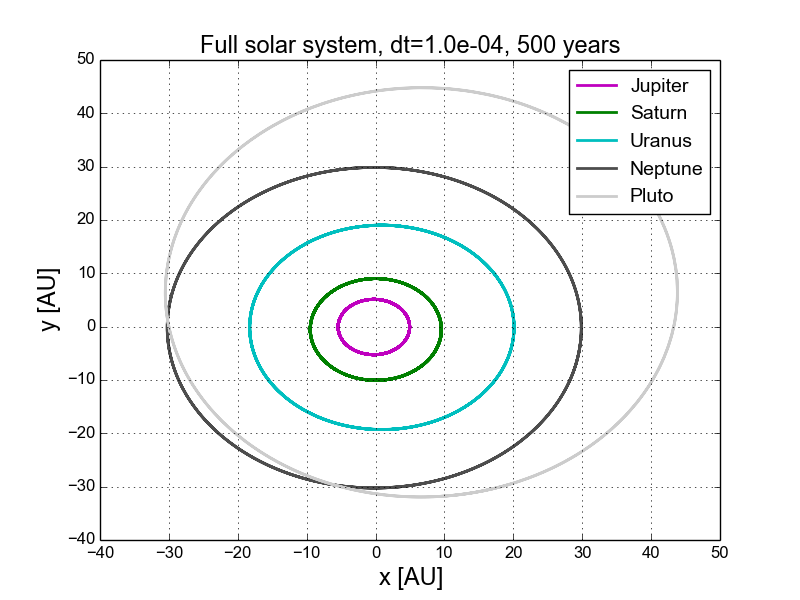
\includegraphics[scale=0.25]{{../figures/WS/pos50_dt1.0e-04_yrs500.0}.png}
\caption{Outer Solar System, $dt = 1.0e-04$}
\label{fig:WSOSS}
\end{subfigure}
\begin{subfigure}{0.33\textwidth}
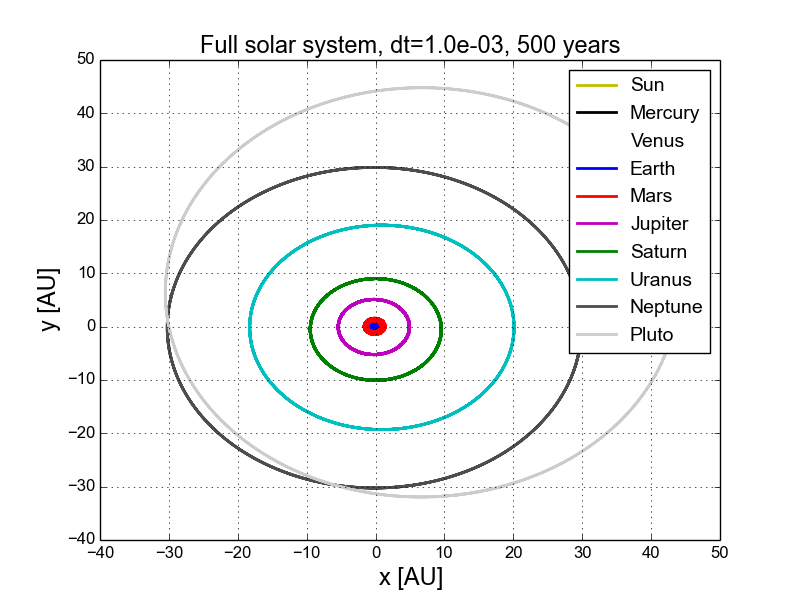
\includegraphics[scale=0.25]{{../figures/WS/pos00_dt1.0e-03_yrs500.0}.png}
\caption{Whole Solar System, $dt = 1.0e-03$}
\label{fig:WSs}
\end{subfigure}
\caption{Simulation of the whole Solar System including Pluto using Velocity Verlet with different time steps. Initial velocity and position for all celestail bodies are retrieved from NASA and the centre-of-mass is in origo. Simulates a time span of 500 years.}
\label{fig:WS}
\end{figure}
\subsubsection*{Perihelion Precession}
By using Verlet twice, first with acceleration given by equation \eqref{eq:FG_comp} and then by the component version of equation \eqref{eq:FgGR}, we could compare the perihelion angles. With dt = $1e-7$, initial velocity in y-direction for Mercury = 12.44 AU/year, initial position for Mercury = (0.3075, 0, 0) and letting the simulation run for a century we found the results presented in figure \ref{fig:perhelion}
\begin{figure}[H]
\centering
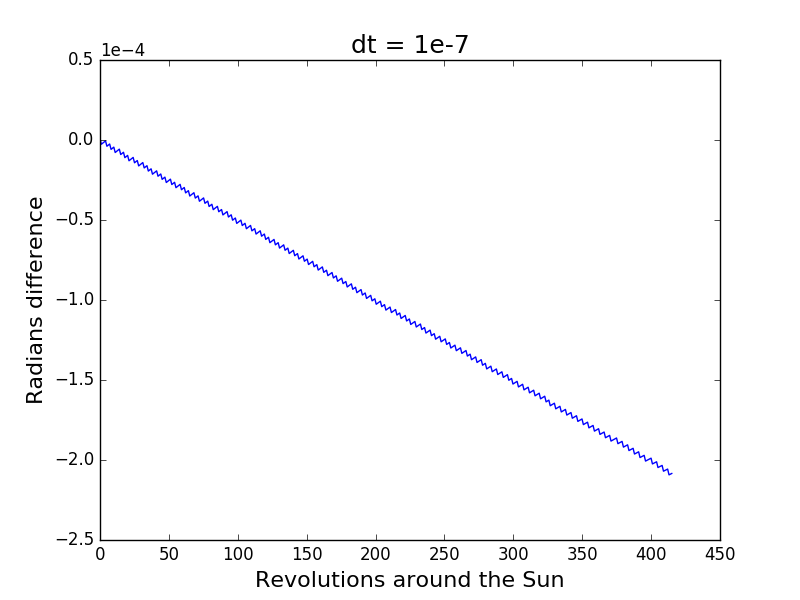
\includegraphics[scale=0.4]{../figures/perheliondt1e-7.png}
\caption{The difference of perhelion angle for the classical and the general relativity case over a century with time step = $1\E{-7}$. The x-axis gives revolutions around the Sun and the y-axis shows the difference in radians.}
\label{fig:perhelion}
\end{figure}
As we can see from figure \ref{fig:perhelion} the difference is about $-2.0 \E{-4}$ after Mercury has revolved about 415 times around the Sun. 
\subsection{Discussion}
As we can see there are several differences between forward Euler and Velocity Verlet. Regarding FLOPs we can see that Euler has less than half of the amount of FLOPs compared to Velocity Verlet. Here it is important to note that the FLOPs we count are only the FLOPs from the method in itself. The program also has calculation of, for example, $a_i$ adding many more FLOPs to the real calculation. However, we want to compare the two methods and have therefore only included the FLOPs from the methods. \\ \\ 
The fact that Velocity Verlet has 11 FLOPs compared to Eulers 4 is again shown by the time usage of the two methods in \husk{Time table!}. Forward Euler uses less time compared to Velocity Verlet, but the effectiveness of the algorithm comes at a price. As we can see throughout the result, Velocity Verlet is the far better alternativ when it comes to accuracy. This is evident from the algorithm where Forward Euler bases its position on a Taylor expansion stopping after the first derivative, Velocity Verlet takes the second derivative into account. The error is therefore dependent on $\mathcal{O}(h^2)$ for forward Euler and $\mathcal{O}(h^3)$ for Velocity Verlet.
\subsubsection*{The Earth-Sun system}
Figures \ref{fig:ES-Euler} and \ref{fig:ES-Verlet} illustrates the difference in accuracy for the two different methods. As we can clearly see, Velocity Verlet is the most accurate. While forward Euler needs $dt = 1.0e-4$ to start being stable, Velocity Verlet is nearly stable at $dt = 1.0e-2$ and stable at $dt = 1.0e-3$. This coincides perfectly with our discussion above. \\ \\
Finding the escape velocity through trial and error is hard. As we can see from figure \ref{fig:ESe8} it seems as though this could be an escape velocity. However, this is not the case. The simulations in figure \ref{fig:ESe} runs for two years, and then stops. If we had run the simulation for an infinite time period, we would see that all velocities below 8.89 AU/year would eventually come back and all equal or above would not. We can say that our numerical results most likely would fit the analytical perfectly if we could simulate an infinite time period, but until the we would get a decreasing escape velocity numerically as we increased the time period.
\subsubsection*{The Earth-Sun-Jupiter system}
The difference in the plots in figure \ref{fig:ESJ1} and \ref{fig:ESJ2} is that the former has the Sun in origo and the latter has center-of-mass in origo. As we can see they are in almost all manners, completely alike. This is because the Sun is so massive that it will stay so close to the center-of-mass even though we don't stick it to origo. By zooming in on the plots in figure \ref{fig:ESJ2} we saw that the Sun did move around origo, but the movement was so small that it would have moved within it's own radius. It is more preciese to let the Sun move because of the gravitational forces from Earth and Jupiter, but it is practically the same as letting it stay in origo. Therefore, it once again depends on what you want to use the program for. If your goal is to study the Sun's movement around the center-of-mass or you need the simulation as preciese as possible, let the Sun move around. If not, you could just keep it still and maybe find a way to not have to calculate the force effecting the Sun and save time. \\

Changing the mass of Jupiter gave us some interesting results. As one can see from figure \ref{fig:ESJ1Crash} the Earth's trajectory is not very abnormal for a Jupiter that is up to 100 times heavier, but increasing the mass to 1000 times normal, gives us the result in \ref{fig:ESJm1000}. Here we can see that the Earth starts out with a relative normal trajectory. But it very soon comes so close to the Sun that it recieves a gravity asist and is, after a little piroutte, shot out of the Solar System. By zooming in close we could see that the Earth would actually crash into the Sun if we had defined the Sun as a 3D object. If we had done this again we would  have made a animation to really get a good view of Jupiters position as it drags the Earth between itself and the Sun.
\subsubsection*{The whole Soalr System}
The whole Solar System, including Pluto as we all love Pluto, is shown in figure \ref{fig:WS}. We had to divide the System into its inner and outer part as the distances traveled by the outer planets are very large compared to those of the inner ones. These simulations were very easily made as our code was already object oriented. When we knew that our smaller system worked, we just added more planets giving by calling the right function and giving them initial position, velocity and mass. This shows one of the great strengths of object oriented programming as we could have added all the celestial bodies we wanted as long as we knew position, velocity and mass by only adding three more lines of code. And as we can see from \ref{fig:WS} the calculations still seems valid even though we have added a lot of planets.
\subsubsection*{Perhelion Precession}
From figure \ref{fig:perhelion} it becomes clear to us that the difference is about $-2.0\E{-4}$ radians after a century. This coincides almost perfectly with the expected value of 43 arcseconds which is the same as $2.1\E{-4}$. (We can neglect the minus sign since we are only interested in the difference.) As we have discussed in the theory, this effect is explained well by general relativity and our results coincides with this as well. Our plot in figure \ref{fig:perhelion} has a little noice and could have been better with a lower $dt$-value. However, this would have taken a long time and since we have a pretty good result with this time resolution, we decided this was good enough. If we were to publish or use the result for something which required high acuracy, we would run the program again with lower $dt$. \\ \\
It has come to our attention that the original mass of Mercury was wrong and we used $2.4\E{23}$ kg when we should have used $3.3 \E{23}$kg. The difference is small, especially as we use per solar mass, and as our results make sense, we are not going to run the program again as we discovered the error very close to finishing the report. If we were to do the project again we would use the right mass, but we are certain it would not give a significantly different result.
\subsection{Conclusion}
\bibliography{references}
\end{document}
